\documentclass{article}\usepackage[]{graphicx}\usepackage[]{color}
%% maxwidth is the original width if it is less than linewidth
%% otherwise use linewidth (to make sure the graphics do not exceed the margin)
\makeatletter
\def\maxwidth{ %
  \ifdim\Gin@nat@width>\linewidth
    \linewidth
  \else
    \Gin@nat@width
  \fi
}
\makeatother

\definecolor{fgcolor}{rgb}{0.345, 0.345, 0.345}
\newcommand{\hlnum}[1]{\textcolor[rgb]{0.686,0.059,0.569}{#1}}%
\newcommand{\hlstr}[1]{\textcolor[rgb]{0.192,0.494,0.8}{#1}}%
\newcommand{\hlcom}[1]{\textcolor[rgb]{0.678,0.584,0.686}{\textit{#1}}}%
\newcommand{\hlopt}[1]{\textcolor[rgb]{0,0,0}{#1}}%
\newcommand{\hlstd}[1]{\textcolor[rgb]{0.345,0.345,0.345}{#1}}%
\newcommand{\hlkwa}[1]{\textcolor[rgb]{0.161,0.373,0.58}{\textbf{#1}}}%
\newcommand{\hlkwb}[1]{\textcolor[rgb]{0.69,0.353,0.396}{#1}}%
\newcommand{\hlkwc}[1]{\textcolor[rgb]{0.333,0.667,0.333}{#1}}%
\newcommand{\hlkwd}[1]{\textcolor[rgb]{0.737,0.353,0.396}{\textbf{#1}}}%
\let\hlipl\hlkwb

\usepackage{framed}
\makeatletter
\newenvironment{kframe}{%
 \def\at@end@of@kframe{}%
 \ifinner\ifhmode%
  \def\at@end@of@kframe{\end{minipage}}%
  \begin{minipage}{\columnwidth}%
 \fi\fi%
 \def\FrameCommand##1{\hskip\@totalleftmargin \hskip-\fboxsep
 \colorbox{shadecolor}{##1}\hskip-\fboxsep
     % There is no \\@totalrightmargin, so:
     \hskip-\linewidth \hskip-\@totalleftmargin \hskip\columnwidth}%
 \MakeFramed {\advance\hsize-\width
   \@totalleftmargin\z@ \linewidth\hsize
   \@setminipage}}%
 {\par\unskip\endMakeFramed%
 \at@end@of@kframe}
\makeatother

\definecolor{shadecolor}{rgb}{.97, .97, .97}
\definecolor{messagecolor}{rgb}{0, 0, 0}
\definecolor{warningcolor}{rgb}{1, 0, 1}
\definecolor{errorcolor}{rgb}{1, 0, 0}
\newenvironment{knitrout}{}{} % an empty environment to be redefined in TeX

\usepackage{alltt}
\IfFileExists{upquote.sty}{\usepackage{upquote}}{}
\begin{document}

\begin{knitrout}
\definecolor{shadecolor}{rgb}{0.969, 0.969, 0.969}\color{fgcolor}\begin{kframe}
\begin{alltt}
\hlkwd{load}\hlstd{(}\hlstr{"SinFigure.RData"}\hlstd{)}
\hlkwd{library}\hlstd{(tidyverse)}
\end{alltt}


{\ttfamily\noindent\itshape\color{messagecolor}{\#\# Loading tidyverse: ggplot2\\\#\# Loading tidyverse: tibble\\\#\# Loading tidyverse: tidyr\\\#\# Loading tidyverse: readr\\\#\# Loading tidyverse: purrr\\\#\# Loading tidyverse: dplyr}}

{\ttfamily\noindent\itshape\color{messagecolor}{\#\# Conflicts with tidy packages ----------------------------------------------}}

{\ttfamily\noindent\itshape\color{messagecolor}{\#\# filter(): dplyr, stats\\\#\# lag():\ \ \ \ dplyr, stats}}\begin{alltt}
\hlkwd{library}\hlstd{(scales)}
\end{alltt}


{\ttfamily\noindent\itshape\color{messagecolor}{\#\# \\\#\# Attaching package: 'scales'}}

{\ttfamily\noindent\itshape\color{messagecolor}{\#\# The following object is masked from 'package:purrr':\\\#\# \\\#\#\ \ \ \  discard}}

{\ttfamily\noindent\itshape\color{messagecolor}{\#\# The following object is masked from 'package:readr':\\\#\# \\\#\#\ \ \ \  col\_factor}}\begin{alltt}
\hlstd{p1} \hlkwb{<-} \hlkwd{ggplot}\hlstd{(df_linear,} \hlkwd{aes}\hlstd{(}\hlkwc{x} \hlstd{= X,} \hlkwc{y} \hlstd{= f))} \hlopt{+} \hlkwd{geom_line}\hlstd{(}\hlkwc{color} \hlstd{=} \hlkwd{muted}\hlstd{(}\hlstr{"blue"}\hlstd{,} \hlnum{70}\hlstd{,} \hlnum{80}\hlstd{),} \hlkwc{size} \hlstd{=} \hlnum{1.1}\hlstd{)} \hlopt{+} \hlkwd{facet_wrap}\hlstd{(}\hlopt{~}\hlstd{method)} \hlopt{+} \hlkwd{stat_function}\hlstd{(}\hlkwc{fun} \hlstd{= g,} \hlkwc{linetype} \hlstd{=} \hlstr{'dashed'}\hlstd{,} \hlkwc{color} \hlstd{=} \hlstr{'black'}\hlstd{)} \hlopt{+} \hlkwd{theme_bw}\hlstd{()} \hlopt{+} \hlkwd{xlab}\hlstd{(}\hlstr{"$x$"}\hlstd{)} \hlopt{+} \hlkwd{ylab}\hlstd{(}\hlstr{"$\textbackslash{}\textbackslash{}widehat f(x)$"}\hlstd{)}
\end{alltt}


{\ttfamily\noindent\color{warningcolor}{\#\# Warning in structure(NULL, class = "{}waiver"{}): Calling 'structure(NULL, *)' is deprecated, as NULL cannot have attributes.\\\#\#\ \  Consider 'structure(list(), *)' instead.}}

{\ttfamily\noindent\color{warningcolor}{\#\# Warning in structure(NULL, class = "{}waiver"{}): Calling 'structure(NULL, *)' is deprecated, as NULL cannot have attributes.\\\#\#\ \  Consider 'structure(list(), *)' instead.}}\begin{alltt}
\hlstd{p2} \hlkwb{<-} \hlkwd{ggplot}\hlstd{(df_sinusoid,} \hlkwd{aes}\hlstd{(}\hlkwc{x} \hlstd{= X,} \hlkwc{y} \hlstd{= f))} \hlopt{+} \hlkwd{geom_line}\hlstd{(}\hlkwc{color} \hlstd{=} \hlkwd{muted}\hlstd{(}\hlstr{"red"}\hlstd{,} \hlnum{70}\hlstd{,} \hlnum{80}\hlstd{),} \hlkwc{size} \hlstd{=} \hlnum{1.1}\hlstd{)} \hlopt{+} \hlkwd{facet_wrap}\hlstd{(}\hlopt{~}\hlstd{method)} \hlopt{+} \hlkwd{stat_function}\hlstd{(}\hlkwc{fun} \hlstd{= f,} \hlkwc{linetype} \hlstd{=} \hlstr{'dashed'}\hlstd{,} \hlkwc{color} \hlstd{=} \hlstr{'black'}\hlstd{)} \hlopt{+} \hlkwd{theme_bw}\hlstd{()} \hlopt{+} \hlkwd{xlab}\hlstd{(}\hlstr{"$x$"}\hlstd{)} \hlopt{+} \hlkwd{ylab}\hlstd{(}\hlstr{"$\textbackslash{}\textbackslash{}widehat f(x)$"}\hlstd{)}
\end{alltt}


{\ttfamily\noindent\color{warningcolor}{\#\# Warning in structure(NULL, class = "{}waiver"{}): Calling 'structure(NULL, *)' is deprecated, as NULL cannot have attributes.\\\#\#\ \  Consider 'structure(list(), *)' instead.}}

{\ttfamily\noindent\color{warningcolor}{\#\# Warning in structure(NULL, class = "{}waiver"{}): Calling 'structure(NULL, *)' is deprecated, as NULL cannot have attributes.\\\#\#\ \  Consider 'structure(list(), *)' instead.}}\begin{alltt}
\hlstd{gridExtra}\hlopt{::}\hlkwd{grid.arrange}\hlstd{(p1, p2,} \hlkwc{ncol} \hlstd{=} \hlnum{1}\hlstd{)}
\end{alltt}


{\ttfamily\noindent\color{warningcolor}{\#\# Warning in structure(NULL, class = "{}waiver"{}): Calling 'structure(NULL, *)' is deprecated, as NULL cannot have attributes.\\\#\#\ \  Consider 'structure(list(), *)' instead.}}

{\ttfamily\noindent\color{warningcolor}{\#\# Warning in structure(NULL, class = "{}waiver"{}): Calling 'structure(NULL, *)' is deprecated, as NULL cannot have attributes.\\\#\#\ \  Consider 'structure(list(), *)' instead.}}

{\ttfamily\noindent\color{warningcolor}{\#\# Warning in structure(NULL, class = "{}waiver"{}): Calling 'structure(NULL, *)' is deprecated, as NULL cannot have attributes.\\\#\#\ \  Consider 'structure(list(), *)' instead.}}

{\ttfamily\noindent\color{warningcolor}{\#\# Warning in structure(NULL, class = "{}waiver"{}): Calling 'structure(NULL, *)' is deprecated, as NULL cannot have attributes.\\\#\#\ \  Consider 'structure(list(), *)' instead.}}

{\ttfamily\noindent\color{warningcolor}{\#\# Warning in structure(NULL, class = "{}waiver"{}): Calling 'structure(NULL, *)' is deprecated, as NULL cannot have attributes.\\\#\#\ \  Consider 'structure(list(), *)' instead.}}

{\ttfamily\noindent\color{warningcolor}{\#\# Warning in structure(NULL, class = "{}waiver"{}): Calling 'structure(NULL, *)' is deprecated, as NULL cannot have attributes.\\\#\#\ \  Consider 'structure(list(), *)' instead.}}

{\ttfamily\noindent\color{warningcolor}{\#\# Warning in structure(NULL, class = "{}waiver"{}): Calling 'structure(NULL, *)' is deprecated, as NULL cannot have attributes.\\\#\#\ \  Consider 'structure(list(), *)' instead.}}

{\ttfamily\noindent\color{warningcolor}{\#\# Warning in structure(NULL, class = "{}waiver"{}): Calling 'structure(NULL, *)' is deprecated, as NULL cannot have attributes.\\\#\#\ \  Consider 'structure(list(), *)' instead.}}

{\ttfamily\noindent\color{warningcolor}{\#\# Warning in structure(NULL, class = "{}waiver"{}): Calling 'structure(NULL, *)' is deprecated, as NULL cannot have attributes.\\\#\#\ \  Consider 'structure(list(), *)' instead.}}

{\ttfamily\noindent\color{warningcolor}{\#\# Warning in structure(NULL, class = "{}waiver"{}): Calling 'structure(NULL, *)' is deprecated, as NULL cannot have attributes.\\\#\#\ \  Consider 'structure(list(), *)' instead.}}

{\ttfamily\noindent\color{warningcolor}{\#\# Warning in structure(NULL, class = "{}waiver"{}): Calling 'structure(NULL, *)' is deprecated, as NULL cannot have attributes.\\\#\#\ \  Consider 'structure(list(), *)' instead.}}

{\ttfamily\noindent\color{warningcolor}{\#\# Warning in structure(NULL, class = "{}waiver"{}): Calling 'structure(NULL, *)' is deprecated, as NULL cannot have attributes.\\\#\#\ \  Consider 'structure(list(), *)' instead.}}

{\ttfamily\noindent\color{warningcolor}{\#\# Warning in structure(NULL, class = "{}waiver"{}): Calling 'structure(NULL, *)' is deprecated, as NULL cannot have attributes.\\\#\#\ \  Consider 'structure(list(), *)' instead.}}

{\ttfamily\noindent\color{warningcolor}{\#\# Warning in structure(NULL, class = "{}waiver"{}): Calling 'structure(NULL, *)' is deprecated, as NULL cannot have attributes.\\\#\#\ \  Consider 'structure(list(), *)' instead.}}

{\ttfamily\noindent\color{warningcolor}{\#\# Warning in structure(NULL, class = "{}waiver"{}): Calling 'structure(NULL, *)' is deprecated, as NULL cannot have attributes.\\\#\#\ \  Consider 'structure(list(), *)' instead.}}

{\ttfamily\noindent\color{warningcolor}{\#\# Warning in structure(NULL, class = "{}waiver"{}): Calling 'structure(NULL, *)' is deprecated, as NULL cannot have attributes.\\\#\#\ \  Consider 'structure(list(), *)' instead.}}

{\ttfamily\noindent\color{warningcolor}{\#\# Warning in structure(NULL, class = "{}waiver"{}): Calling 'structure(NULL, *)' is deprecated, as NULL cannot have attributes.\\\#\#\ \  Consider 'structure(list(), *)' instead.}}

{\ttfamily\noindent\color{warningcolor}{\#\# Warning in structure(NULL, class = "{}waiver"{}): Calling 'structure(NULL, *)' is deprecated, as NULL cannot have attributes.\\\#\#\ \  Consider 'structure(list(), *)' instead.}}

{\ttfamily\noindent\color{warningcolor}{\#\# Warning in structure(NULL, class = "{}waiver"{}): Calling 'structure(NULL, *)' is deprecated, as NULL cannot have attributes.\\\#\#\ \  Consider 'structure(list(), *)' instead.}}

{\ttfamily\noindent\color{warningcolor}{\#\# Warning in structure(NULL, class = "{}waiver"{}): Calling 'structure(NULL, *)' is deprecated, as NULL cannot have attributes.\\\#\#\ \  Consider 'structure(list(), *)' instead.}}\end{kframe}

{\centering 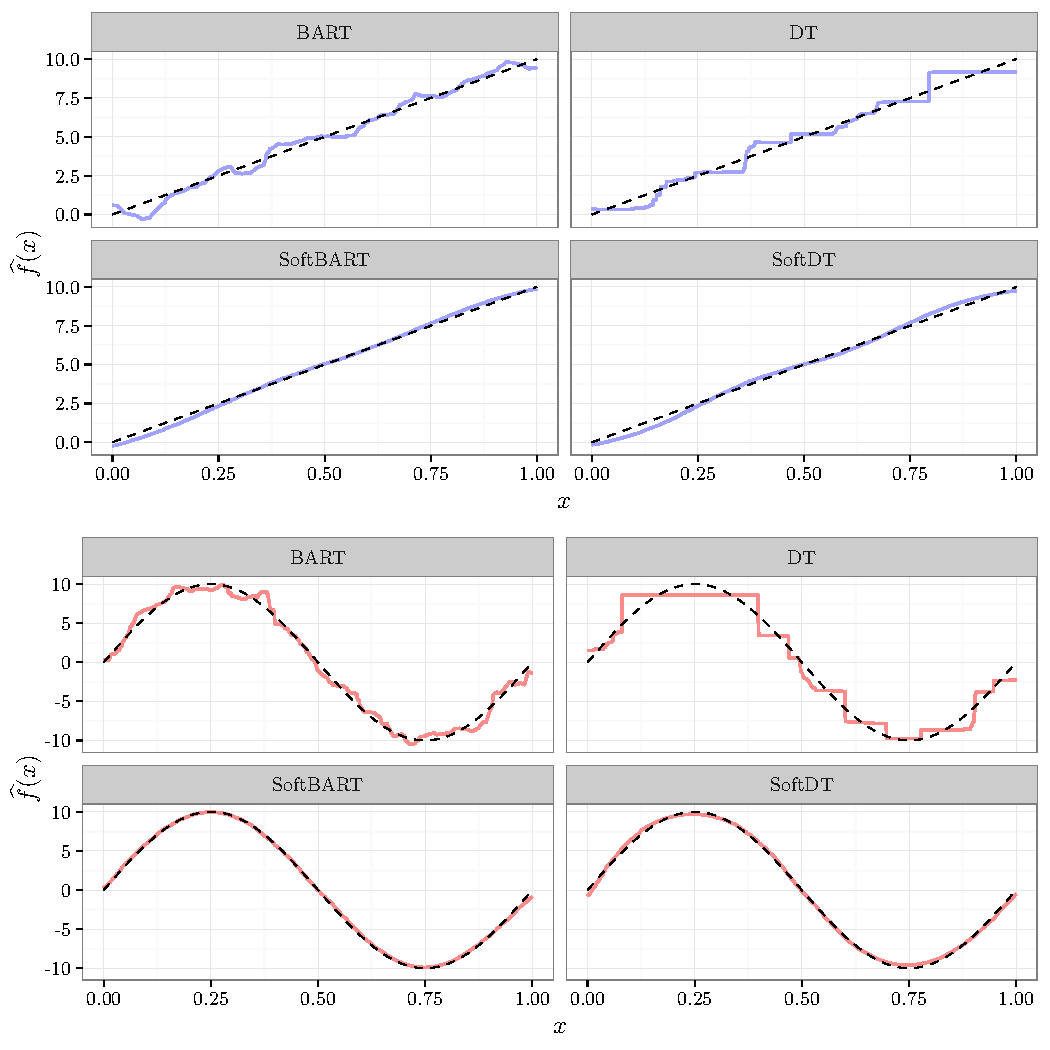
\includegraphics[width=\textwidth]{figure/simple-functions-1} 

}



\end{knitrout}


\end{document}
